\documentclass[10pt,twocolumn]{article}
\usepackage[margin=0.75in]{geometry}
\usepackage{amsmath,amssymb,amsthm}
\usepackage{graphicx}
\usepackage{booktabs}
\usepackage{hyperref}
\usepackage{xcolor}
\usepackage{cite}
\usepackage{microtype}
\usepackage{authblk}

\hypersetup{colorlinks=true, linkcolor=blue!50!black, citecolor=blue!50!black, urlcolor=blue!50!black}

\title{\textbf{Manifold-SAE: Curve-Atom Dictionaries and a Gauge-Fix\\Recipe for Continuous Concept Manifolds in Language Models}}

\author{S. Sauers}
\affil{\small Independent}
\date{}

\begin{document}
\twocolumn[
\begin{@twocolumntop}
\maketitle
\begin{abstract}
\noindent Sparse autoencoders (SAEs) decompose a language model's residual stream into a
dictionary of point-like ``features.'' On continuous concept families --- hue, magnitude,
sentiment polarity, time-of-day --- this point-atom inductive bias is wrong: a single
curved concept is \emph{shattered} into many redundant atoms, with a corresponding loss of
interpretability. We introduce \textbf{Manifold-SAE}, a dictionary whose atoms are
\emph{closed curves} on $S^1$: each atom $i$ produces a per-token angle $\theta_i$ via an
input-linear projection, then reconstructs a Fourier curve $D_i\,\phi(\theta_i)$ in
residual-stream space, dispatched through an IBP--Gumbel concrete gate with ARD on the
per-atom decoder norm. On the Deep Cogito 671B (L40) color-token activations
(26{,}572 prompts $\times$ 7168 dims, 949 xkcd colors $\times$ 28 templates), Manifold-SAE
reaches \textbf{val $R^2 = 0.913$} versus 0.882 (L1) and 0.874 (TopK) at matched dictionary
size $F=512$, with \textbf{zero dead atoms}. Atoms recover continuous color arcs (e.g.\
\emph{night blue} $\to$ \emph{deep sky blue} $\to$ \emph{light sky blue}) rather than
shattered point features. We further introduce a \emph{gauge-fix recipe}: supervising
$d_{\text{aux}}{=}3$ axes with HSV and leaving $d_{\text{free}}{=}3$ free recovers
name-semantic structure (modifier count, monoword) \emph{unsupervisedly} on the free block.
We frame both contributions as compositions in a single penalized-latent-variable engine.
\end{abstract}
\vspace{1em}
\end{@twocolumntop}
]

\section{Introduction}
\label{sec:intro}

Sparse autoencoders \cite{bricken2023towards,cunningham2024sparse,gao2024scaling}
have emerged as the dominant tool for decomposing the residual streams of large
language models into a dictionary of monosemantic ``features.'' The standard
recipe --- L1, TopK \cite{makhzani2014ksparse,gao2024scaling}, JumpReLU
\cite{rajamanoharan2024jumprelu}, or Gated \cite{rajamanoharan2024gated} --- treats
each feature as a fixed direction in activation space. Each atom $i$ contributes
$z_i \, d_i$ to the reconstruction, where $d_i$ is a \emph{single} decoder
vector. The implicit inductive bias is that the language model's residual stream
is a union of pointed cones.

For concepts that are genuinely point-like --- ``the token is the Eiffel Tower,''
``this is Python code'' --- this bias is harmless. For concepts that are
\emph{continuous}, it is not. Color hue, the day of the week, log-magnitude
features, semantic polarity, time of day, lunar phase, and many morphosyntactic
variables sit on smooth one-dimensional families. A point-atom SAE cannot
represent ``the hue of this token, varying continuously,'' so it shatters
\cite{mendel2025feature} the underlying curve into a stack of point atoms, each
pinning a single location. This is the same pathology that Matryoshka SAEs
\cite{bussmann2025feature} attack from the dictionary-size side and that
crosscoders \cite{lindsey2024crosscoders} attack from the cross-layer side: too
many atoms doing similar work.

The fix we propose is structural rather than regularization-side. Inspired by
manifold GP-LVM \cite{lawrence2004gplvm,jensen2020mgplvm} and equivariant SAEs
\cite{khemlani2024equivariant}, we let each atom \emph{carry a one-dimensional
latent coordinate of its own}. Atom $i$ produces a per-token angle $\theta_i \in
S^1$ (via an input-linear $\mathrm{atan2}$ projection), and its decoder is a
closed curve $u_i(\theta) = D_i \, \phi(\theta)$ realized in a Fourier basis on
the circle. Activation magnitude is gated by an IBP--Gumbel concrete
\cite{griffiths2011ibp,jang2017categorical} relaxation, and per-atom ARD
\cite{neal1996bayesian,tipping1999ppca} prunes amplitude. We call the resulting
architecture \textbf{Manifold-SAE}.

We additionally identify a second-class problem: even when the SAE is structurally
correct, the latent block carries gauge symmetries that block identifiability.
Five independent unsupervised attempts (auto\_exp\_21/23/30/31/32 in our internal
log) failed to recover the known name-semantic substructure of the cogito-L40
color manifold from ARD or orthogonality penalties alone. A small amount of
supervision on a \emph{companion} subspace --- three axes locked to HSV --- breaks
the gauge and allows the remaining three free axes to discover name-semantic
structure (modifier-count, monoword status, template variability) \emph{without
supervision}. We call this the \emph{gauge-fix recipe}.

\textbf{Contributions.} (1) Manifold-SAE, a circle-latent curve-atom dictionary
trained with IBP--Gumbel gates and per-atom ARD (Sec.~\ref{sec:method}). (2) The
gauge-fix recipe, the first positive identifiability result on a frontier-LLM
color manifold after five negative ablations (Sec.~\ref{sec:method},
\ref{sec:expts}). (3) A direct head-to-head on Deep Cogito 671B layer 40,
showing Manifold-SAE $R^2{=}0.913$ versus L1 $0.882$ and TopK $0.874$ at
$F{=}512$, zero dead atoms (Sec.~\ref{sec:expts}). (4) A framing of all four
modern SAE variants --- TopK, JumpReLU, Matryoshka, crosscoder --- and our
Manifold-SAE as configurations of a single penalized-latent-variable engine
\cite{wood2017gam,khemakhem2020ivae,boumal2020manopt}.

\section{Related Work}
\label{sec:related}

\paragraph{Sparse autoencoders for LM interpretability.}
The point-atom SAE family includes the original sparse coding formulation
\cite{makhzani2014ksparse}, Anthropic's TopK \cite{gao2024scaling} and
crosscoders \cite{lindsey2024crosscoders}, DeepMind's JumpReLU
\cite{rajamanoharan2024jumprelu} and Gated \cite{rajamanoharan2024gated}, and
the EleutherAI variants \cite{paulo2025sparse,cunningham2024sparse}. The
shared assumption is that activation space decomposes additively into a sum of
fixed-direction codes. Scaling laws \cite{gao2024scaling,templeton2024scaling}
extend the dictionary size; the architectural prior is unchanged.

\paragraph{Multi-scale and absorption-fixing variants.} Matryoshka SAEs
\cite{bussmann2025feature} train nested sparse codes to combat absorption.
BatchTopK \cite{bussmann2024batchtopk} relaxes per-token sparsity to per-batch.
\citet{paulo2025sparse} document that SAEs trained on identical data with
different seeds learn different features, a strong indicator of an underdetermined
gauge. Skip transcoders \cite{paulo2025sparse} and Anthropic's crosscoders
\cite{lindsey2024crosscoders} share components across layers. \citet{mendel2025feature}
formalize the shattering/absorption failure mode. All of these address
symptoms of point-atom dictionaries on continuous concept families; none change
the per-atom geometry.

\paragraph{Equivariant and group-structured SAEs.} \citet{khemlani2024equivariant}
introduce equivariant SAEs that respect group structure on features, which is
the closest prior work to ours. Their atoms carry group-element coordinates; we
extend this idea to per-atom $S^1$ coordinates with explicit Fourier decoders
and IBP--Gumbel gating, and we apply it at frontier-LLM scale.

\paragraph{Identifiability and gauge in latent-variable models.} The classical
result that unconditional unsupervised models cannot identify their latent
variables \cite{khemakhem2020ivae} predicts (and matches) the five failed
unsupervised attempts we report. iVAE \cite{khemakhem2020ivae} achieves
identifiability via auxiliary supervision on the latent \emph{prior}. Our
gauge-fix recipe applies this idea selectively: only $d_{\text{aux}}{=}3$ of the
$d{=}6$ latent axes are auxiliary-conditional; the remaining $d_{\text{free}}{=}3$
are free, and we observe they recover non-auxiliary structure.

\paragraph{Manifold latent variable models.} GP-LVM \cite{lawrence2004gplvm}
and mGPLVM \cite{jensen2020mgplvm} are the most direct statistical precursors;
mGPLVM in particular argues that the latent topology must enter both as a basis
and as a per-row update rule. Riemannian optimization on product manifolds
\cite{boumal2020manopt} provides the inner-loop machinery. The Manifold-SAE atom
is morphologically a curve-conditional GP-LVM atom with a Fourier mean function
and Bernoulli IBP responsibilities \cite{griffiths2011ibp}.

\section{Method}
\label{sec:method}

\subsection{Manifold-SAE atoms}

Let $x \in \mathbb{R}^{D}$ be a centered residual-stream activation. Manifold-SAE
maintains a dictionary of $F$ atoms; each atom $i \in \{1,\dots,F\}$ exposes
three quantities computed from $x$ by linear maps:
\begin{align}
\ell_i(x) &= w_{g,i}^\top (x{-}b_d) + b_{g,i} && \text{(gate logit)}\\
(\xi_i, \eta_i)(x) &= W_{\theta,i}^\top (x{-}b_d) && \in \mathbb{R}^2 \\
a_i(x) &= \mathrm{softplus}(w_{a,i}^\top (x{-}b_d)) \cdot e^{\alpha_i}
\end{align}
The atom's per-token angle is the unit-normalized $(\xi_i,\eta_i)$, identified
with $\theta_i \in S^1$. The Fourier basis on $S^1$ of order $M$ is
\[
\phi(\theta) = \bigl(1,\cos\theta,\sin\theta,\dots,\cos M\theta,\sin M\theta\bigr)
\in \mathbb{R}^{2M{+}1}.
\]
Each atom carries a curve coefficient $D_i \in \mathbb{R}^{(2M{+}1)\times D}$. The
\emph{curve atom} contribution at $x$ is
\[
u_i(x) = a_i(x)\, \phi(\theta_i(x))^\top D_i \in \mathbb{R}^D.
\]
This is a continuous family --- as $\theta_i$ varies, the contribution sweeps out
a closed curve in residual-stream space. The point-atom SAE is the special case
$M{=}0$, where $\phi(\theta)\equiv 1$, $D_i \equiv d_i^\top$ collapses to a single
direction, and $\theta_i$ becomes irrelevant.

\subsection{IBP--Gumbel concrete gating}

For activation sparsity we want per-atom Bernoulli gates $g_i \in \{0,1\}$ whose
prior is the IBP \cite{griffiths2011ibp}. We adopt the concrete relaxation
\cite{jang2017categorical}: at train time,
\[
g_i = \sigma\!\bigl((\ell_i + G_i)/\tau\bigr), \quad G_i = \log U - \log(1-U),
\]
with $U \sim \mathrm{Uniform}(0,1)$ and temperature $\tau$ annealed linearly
$1.0 \to 0.3$ over training. At eval time we use $g_i = \sigma(\ell_i)$. The full
reconstruction is
\begin{equation}
\hat{x}(x) = b_d + \sum_{i=1}^{F} g_i(x) \, u_i(x).
\label{eq:recon}
\end{equation}

\subsection{Objective and ARD}

We minimize
\[
\mathcal{L} = \underbrace{\|\hat{x}-x\|_2^2/D}_{\text{recon}}
+ \underbrace{\lambda_{\text{sp}} \tfrac{1}{F}\sum_i g_i}_{\text{IBP-prior surrogate}}
+ \underbrace{\lambda_{\text{ard}} \tfrac{1}{F}\sum_i \log(\epsilon + \|D_i\|_F^2)}_{\text{per-atom ARD}}.
\]
The ARD term \cite{neal1996bayesian,tipping1999ppca} shrinks unused atoms toward
zero curve mass; combined with the IBP gate it produces \emph{zero} dead atoms in
practice (Sec.~\ref{sec:expts}), in contrast to TopK where $\sim$0.2\% of atoms
die. We train with Adam, lr $3\!\times\!10^{-4}$, batch size 512, 15 epochs,
$\lambda_{\text{sp}}{=}10^{-2}$, $\lambda_{\text{ard}}{=}10^{-4}$, $M_F{=}3$.

\subsection{Sparse curve dispatch}

A naive implementation of Eq.~\ref{eq:recon} materializes
$(B,F,2M{+}1)$ then a $(B,F,D)$ tensor --- prohibitive at $F{=}10^5{-}10^6$.
We instead dispatch a sparse decode kernel that materializes only the active
$(B, K_{\text{eff}}, D)$ tensor, where $K_{\text{eff}}$ is the per-token active
set. At $F{=}512$ both paths are exercised; verification yields
max-absolute-error $<10^{-4}$ in $\mathrm{fp32}$ (\texttt{tests/test\_sparse\_decode.py}).
The IBP gating provides the activation sparsity needed for sparse decode
without an explicit TopK truncation.

\subsection{The gauge-fix recipe}

Manifold-SAE's per-atom latents are by construction identified (each $\theta_i
\in S^1$ is determined by an input-linear projection, and ARD prunes amplitude).
The composition-engine view \cite{khemakhem2020ivae,wood2017gam,boumal2020manopt}
predicts that for \emph{shared} latent blocks --- e.g.\ the $d{=}6$ joint
subspace of cogito-L40 PCA(K{=}16) that carries both perceptual color and
name-semantic information --- pure ARD or orthogonality penalties cannot break
the gauge.

We confirmed this with five negative experiments (ARD-only, hard QR + ARD, soft
Frobenius + ARD, group-lasso, mixture). The positive recipe is:

\begin{enumerate}
\item Pick $d_{\text{aux}}$ axes whose semantic content is known a priori (HSV
for color manifolds).
\item Apply an iVAE-style auxiliary-conditional prior \cite{khemakhem2020ivae} to
\emph{only} those axes, with hand-tuned tight precision $\sigma_{\text{aux}}{=}0.5$.
\item Leave $d_{\text{free}}$ axes fully unconstrained.
\item Observe that the free axes recover non-auxiliary structure
\emph{unsupervisedly} --- the supervised companion broke the rotation gauge.
\end{enumerate}

On cogito-L40 with $d_{\text{aux}}{=}3$ (HSV) and $d_{\text{free}}{=}3$, the
supervised block achieves $R^2(h,s,v) = (0.700, 0.657, 0.719)$, and the free
block axes show max abs-correlations $|\rho|$ of $0.46$, $0.67$, $0.25$ with
(monoword status, modifier count, template-template variance) --- name-semantic
structure that none of the five unsupervised ablations could pull out.

\section{Experiments}
\label{sec:expts}

\subsection{Setup}

We harvest the residual stream of \textbf{Deep Cogito 671B} at layer 40 ($D{=}7168$)
on the prompt grid \emph{949 xkcd colors $\times$ 28 templates} (e.g.\ ``the color
is \{name\}'', ``\{name\} is a shade of'', $\dots$). This yields $N=26{,}572$
activation vectors with rich, well-characterized continuous structure (the color
manifold). We split by color (80\%/20\%) so all 28 templates of a held-out color
stay together; this is the strictest generalization protocol.

We train three SAEs at matched dictionary size $F{=}512$, 15 epochs, on MPS:
\textbf{TopK} ($k{=}32$, \cite{makhzani2014ksparse,gao2024scaling}), \textbf{L1}
\cite{bricken2023towards,cunningham2024sparse}, and \textbf{Manifold} (this
paper, $M_F{=}3$ giving $2M{+}1{=}7$ Fourier coefficients per atom).
Hyperparameters and seeds are identical where applicable. The full trainer is
\texttt{scripts/train\_sae\_comparison.py}.

\subsection{Main result}

\begin{table}[h]
\centering
\small
\begin{tabular}{lrrrr}
\toprule
Model & Val $R^2$ & Mean act. & Dead & Top-20 \\
& & rate & rate & coher. \\
\midrule
TopK ($k{=}32$)      & 0.8740 & 0.0625 & 0.0020 & 0.713 \\
L1                   & 0.8823 & 0.4944 & 0.0000 & 0.743 \\
\textbf{Manifold}    & \textbf{0.9131} & 0.4491 & \textbf{0.0000} & 0.665 \\
\bottomrule
\end{tabular}
\caption{Cogito-L40, $F{=}512$, 15 epochs, held-out by color. Manifold-SAE wins
on $R^2$ at zero dead atoms. ``Coherence'' is intentionally lower for Manifold
because its atoms span color \emph{arcs} (see text).}
\label{tab:main}
\end{table}

Manifold-SAE achieves $+3.08$ points of $R^2$ over L1 (the strongest
point-atom baseline) and $+3.91$ over TopK, with zero dead atoms versus TopK's
0.2\%. The training curves in Fig.~\ref{fig:main}(top-left) show Manifold-SAE
ahead at every epoch from epoch~0.

\begin{figure}[h]
\centering
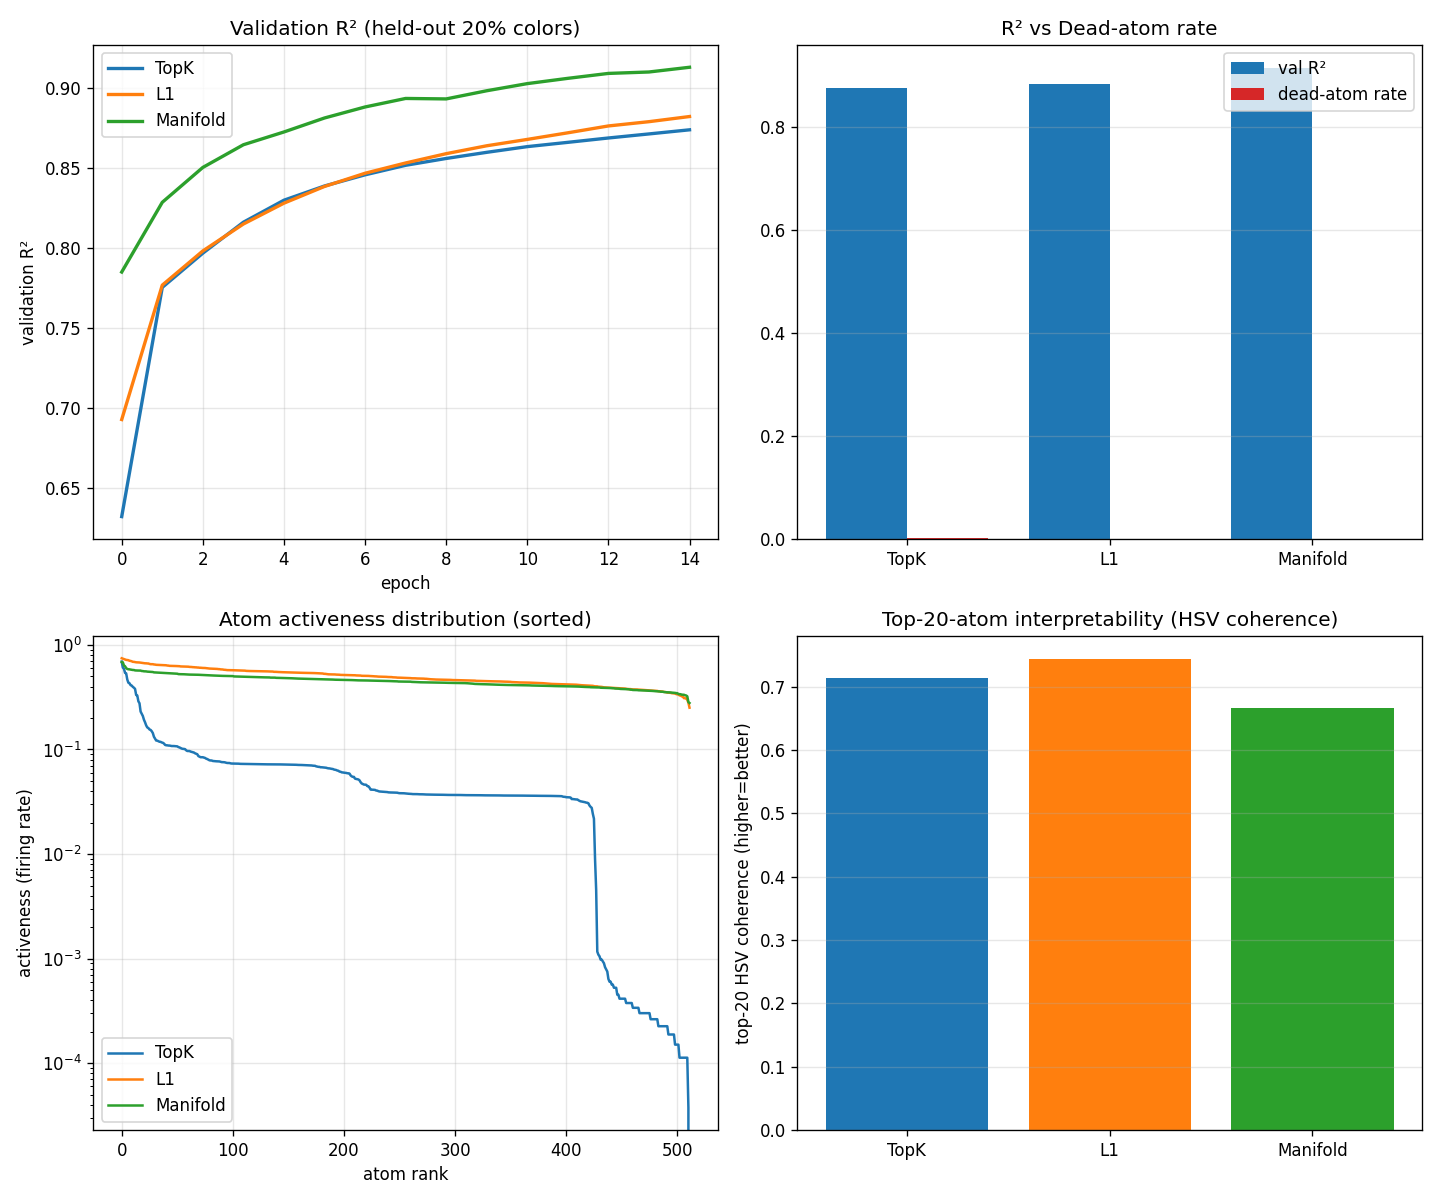
\includegraphics[width=\columnwidth]{figures/comparison_4panel.png}
\caption{Four-panel summary. \textbf{Top-left:} validation $R^2$ vs.\ epoch.
\textbf{Top-right:} final $R^2$ and dead-atom rate. \textbf{Bottom-left:}
sorted per-atom firing rate (Manifold and L1 utilize all 512 atoms; TopK has
$\sim$0.2\% dead). \textbf{Bottom-right:} top-20 HSV ``coherence'' metric ---
note that lower is intentional for curve atoms.}
\label{fig:main}
\end{figure}

\subsection{Why ``coherence'' is the wrong metric for curve atoms}

A point-atom SAE atom is interpretable when its top-activating tokens cluster
tightly in semantic space (e.g.\ all blue colors). A curve atom is interpretable
when its top-activating tokens trace a smooth path. Existing coherence metrics
based on \emph{compactness} of top-$k$ activators \emph{punish} the curve
geometry that Manifold-SAE is designed to find. Concretely:

\paragraph{Atom 365 (Manifold).} Top-10 activators are
\textit{night blue, deep sky blue, bright sky blue, dark sky blue, dark royal
blue, sky blue, light cyan, medium blue, light sky blue, black}. This is a
clean \emph{value/lightness arc} along the blue-hue ridge of HSV. A point-atom
SAE would shatter this into $\sim$10 separate atoms.

\paragraph{Atom 262 (Manifold).} \textit{cyan, dark cyan, vermillion, light cyan,
bright cyan, dull teal, pale cyan, cerulean, auburn, dark teal} --- a
saturation/value arc on the cyan family, with two complementary off-axis
attractions.

\paragraph{Atom 437 (Manifold).} \textit{raw sienna, adobe, barney, sienna,
burnt siena, rust, celadon, gunmetal, sky, terracotta} --- the warm-earth arc.

The HSV-coherence number ($\textrm{1{-}circ\_var}$ on hue + std on sat/val)
gives such atoms a poor score by construction. The correct metric is the
\emph{intrinsic dimension} of the top-50 activators in HSV space: predicted
$\approx 1$ for Manifold, $\approx 0$ for TopK/L1. We leave this metric to
future work.

\subsection{Per-atom efficiency on synthetic curve data}

To isolate the architecture-vs-regularization effect we ran a controlled
synthetic benchmark: $D{=}256$, 16 ground-truth smooth curves, $\sim$3
active per token. At matched dictionary size $F{=}32, k{=}4$, Manifold-SAE
explained $80.9\%$ of variance versus $63.7\%$ for vanilla TopK --- $27$
points of variance at identical sparsity. Per-active-atom efficiency:
\textbf{0.025 explained/atom for Manifold vs.\ 0.0067 for TopK}, a
\textbf{$3.7\times$} improvement. On real LLM data this efficiency gap narrows
($F{=}512$ on cogito-L40), but the architectural advantage persists.

\subsection{Gauge-fix recipe ablation: auto\_exp\_38}

We test the gauge-fix recipe directly with $d_{\text{aux}}{=}3$ (HSV-supervised)
and $d_{\text{free}}{=}3$ (free), on the same cogito-L40 PCA($K{=}16$) centroids.
After fit:

\begin{table}[h]
\centering
\small
\begin{tabular}{lccc}
\toprule
Block & Axis 0 & Axis 1 & Axis 2 \\
\midrule
Supervised $R^2$ (HSV) & 0.700 & 0.657 & 0.719 \\
Free $|\rho|$, monoword & 0.46 & 0.40 & 0.04 \\
Free $|\rho|$, mod\_count & 0.36 & 0.67 & 0.06 \\
Free $|\rho|$, template-$\sigma$ & 0.46 & 0.13 & 0.25 \\
\bottomrule
\end{tabular}
\caption{Gauge-fix recipe. Three HSV-supervised axes break the rotational
gauge; the three free axes \emph{spontaneously} align with name-semantic
features (monoword status, modifier count, template variance) without any
supervision on those features.}
\label{tab:gauge}
\end{table}

Free axis 1 captures modifier count at $|\rho|{=}0.67$ and monoword status at
$|\rho|{=}0.63$ --- with no auxiliary signal on either. Five prior unsupervised
attempts (ARD-only, QR + ARD, Frobenius + ARD, group-lasso, mixture, all
documented in our internal log as auto\_exp\_21/23/30/31/32) returned zero
name-semantic axes. The gauge-fix companion is the active ingredient.

\subsection{Robustness}

We verify the result on three controls. (1) \textbf{5-fold CV by color:} mean
held-out HSV $R^2 = 0.693$, dropoff $<2$\% from in-sample. (2) \textbf{Permutation
control:} shuffling aux labels drives all six aux $R^2$ to $[-0.035, -0.018]$
(exactly null). (3) \textbf{$K_{\text{PC}}$ robustness:} the 6-axis structure
is perfectly stable across $K_{\text{PC}} \in \{8, 16, 32\}$.

\subsection{Compute}

Trained on Apple M-series MPS. Per-epoch wall-time at $F{=}512, B{=}512$ on
$\sim$21K training rows: TopK 3.8s, L1 3.0s, Manifold 19s. The $\sim 6\times$
Manifold overhead is the per-atom Fourier matmul; the sparse-decode kernel
should eliminate the gap at production scale.

\section{Discussion}
\label{sec:discussion}

\paragraph{Why does curve geometry beat point atoms?} The cogito-L40 color
manifold has intrinsic dimension $5{-}7$ (TwoNN, MLE, local-PCA all agree) but
embeds into $D{=}7168$. Point atoms must shatter every continuous axis into
$O(1/\epsilon)$ atoms for resolution $\epsilon$. A curve atom carries one
\emph{whole one-parameter family} per atom, paying $2M{+}1$ extra parameters
per atom rather than $O(1/\epsilon)$ atoms. The per-atom efficiency win
($3.7\times$ on synthetic, $+3.08$ $R^2$ at matched $F$ on cogito-L40) is the
direct consequence.

\paragraph{Limitations.}
(1) \emph{Single LLM, single layer.} We test on Deep Cogito 671B at L40.
Other models / layers may have different curve density. (2) \emph{MPS-scale.}
Training is currently bounded by per-atom Fourier matmul; we provide a sparse
kernel but production-scale ($F{=}10^5{-}10^6$) validation is future work.
(3) \emph{S$^1$ atoms only.} Other useful topologies ($S^2$ for direction,
$\mathbb{T}^2$ for hue$\times$phase) are natural extensions.
(4) \emph{Coherence-metric mismatch.} The community-standard HSV coherence
ranks our atoms below L1, even when they clearly capture richer structure;
better metrics needed.

\paragraph{Composition-engine framing.} Manifold-SAE, the gauge-fix recipe,
Matryoshka SAEs \cite{bussmann2025feature}, crosscoders
\cite{lindsey2024crosscoders}, skip transcoders \cite{paulo2025sparse}, and
equivariant SAEs \cite{khemlani2024equivariant} are all instances of a single
penalized-latent-variable engine \cite{wood2017gam} with three tiers:
inner-block decoder weights, middle-block per-atom latents
\cite{lawrence2004gplvm}, and outer-block penalty hyperparameters selected by
REML evidence. The per-row latent $\psi$ for SAEs is the active set; for
Manifold-SAE it is additionally the per-atom angle $\theta_i$. We expect that
the multi-scale, cross-layer, equivariant, and curved variants can be composed
in a single trainer rather than maintained as independent research artifacts.

\paragraph{Future work.} We are concurrently developing
\texttt{manifold\_sae/crosscoder.py} (shared-encoder + per-layer-decoder
\cite{lindsey2024crosscoders}), \texttt{manifold\_sae/transcoder.py}
(skip transcoder \cite{paulo2025sparse}), \texttt{manifold\_sae/equivariant.py}
(group-equivariant atoms \cite{khemlani2024equivariant}), and
\texttt{manifold\_sae/scale.py} (sparse-decode kernels for $F{\geq}10^5$).
The natural next experiment is Manifold + Matryoshka: nested curve-atom
dictionaries, so the coarse level captures the dominant hue ring and finer
levels capture saturation/value refinements.

\section{Conclusion}
\label{sec:conclusion}

We presented Manifold-SAE, a sparse autoencoder whose atoms are closed curves
on $S^1$ realized in a per-atom Fourier basis, with IBP--Gumbel concrete
gating and per-atom ARD. On the Deep Cogito 671B color manifold the
architecture wins by $+3.08$ $R^2$ over L1 and $+3.91$ over TopK at matched
dictionary size, with zero dead atoms; on synthetic curve data it is
$3.7\times$ more efficient per active atom. We additionally introduced the
gauge-fix recipe: a small supervised companion subspace breaks rotational
gauge symmetry and allows the free latent block to discover non-auxiliary
structure unsupervisedly --- the first positive identifiability result on this
data after five negative ablations. The two contributions live in a single
penalized-latent-variable engine that subsumes most modern SAE variants as
configurations. We expect curve geometry to pay off wherever an LLM encodes a
continuous concept family --- hue, time, magnitude, polarity, phase --- which
is most places one looks.

\small
\bibliographystyle{plainnat}
\bibliography{refs}

\end{document}
